\chapter{Signal formation in germanium detectors}
\label{cha:detector}
When particles ($\alpha, \beta, \gamma, n, p$, etc.) interact inside
the germanium semiconductor detector, they create electron-hole pairs,
which act as charge carriers. Due to the electric field inside the
detector the charge carriers drift and induce electric signals in
electrodes. The electric signals are amplified, digitized and recorded
by the electronics and data acquisition systems connected to the
germanium detector. The whole process of signal formation in germanium
detectors and their supporting electronics is briefly reviewed in this
chapter.

\section{Interactions of radiation with matter}
\label{sec:det:phys}

\subsection{Electrons and positrons}
\label{sec:det:ep}
Electrons and positrons traversing matter lose their kinetic energy
mainly by two processes, ionization and bremsstrahlung. High energy
(GeV range) electrons and positrons predominantly lose energy by
bremsstrahlung. Low energy (MeV range) electrons and positrons
predominantly lose energy by ionization. The energy at which an
electron or a positron loses as much energy in collisions as in
radiation is called critical energy $\epsilon$. For elements with
charge $Z > 13$ the critical energy is \cite{Ama81}
\begin{equation}
\label{eq:det:ecrit}
\epsilon = (550/Z) \text{ MeV}.
\end{equation}
For germanium $\epsilon \approx 17$~MeV. Hence, electrons emitted from
the double beta decay of $^{76}$Ge mainly loss their energy by
ionization.

The range of electrons and positrons depends on their energy and the
material they traverse (see Ref.~\cite{Bri84} and references
therein). The average range of a 1~MeV electron in germanium is about
0.5~mm.

After a positron has lost all its kinetic energy, it annihilates with
an electron into two photons with an energy of 511~keV each,
corresponding to the rest mass of electrons.

\subsection{Photons}
\label{sec:det:gamma}
Photons emitted by radioactive isotopes have energies ranging from
several keV to several MeV. The possible interaction processes of
photons in matter are photoelectric effect, Compton (incoherent)
scattering, Rayleigh (coherent) scattering and pair production. Since
Rayleigh scattering does not change the energy of the scattered photon
but only its momentum, it is not relevant for GERDA.

\textbf{Photoelectric effect:} When a photon interacts with an atom,
its entire energy may be transferred to an atomic shell electron which
leaves the shell. The energy of the secondary electron is equal to the
difference of the incident photon energy and the binding energy of the
electron. If the electron originates from an inner shell of the atom,
an outer shell electron fills the vacancy. Consequently, either
characteristic x-rays are emitted, or, if the x-ray photons are
re-absorbed, secondary Auger-electrons are emitted. The cross section
of the photoelectric effect is inversely proportional to the photon
energy. Hence, the photoelectric effect is the main interaction
mechanism for photons at low energy (up to about 200~keV for Ge).

\textbf{Compton scattering:} A photon scatters on a weakly bound
electron (quasi-free), transferring only part of its energy and
momentum. The angular distribution of the scattered photons is
described by the Kein-Nishina formula. The maximum energy transfer
occurs when the incident photon is scattered by $180^{\circ}$. Compton
scattering is the predominant interaction process for photons of
energies between about 200~keV and 8~MeV for germanium. A 1.33~MeV
photon undergoes on average three Compton scatterings before being
absorbed through the photoelectric effect. The mean free path of such
a photon is about three centimeters.

\textbf{Pair production:} If the photon energy exceeds twice the rest
mass of the electron, the photon can create an electron-positron pair
in the electric field of a nucleus. The rest of the photon energy is
transferred to the created electron and positron as kinetic energy. A
significant cross section for this interaction mechanism arises only
for energies above $4\sim5$~MeV.

\subsection{Neutrons}
\label{sec:det:neutron}
Because of the lack of charge, neutrons have a relatively high
penetration power. However, there are five processes that occur when
neutrons interact with nuclei depending on the kinetic energy of the
incident neutrons:

\textbf{Capture:} The nucleus, Z, absorbs the incident neutron, $n$,
and de-excites with the emission of one or more photons, denoted as
$^{\text{A}}$Z$(n,\gamma)$, where A is the atomic number of the
nucleus. In case of \textbf{internal conversion} an electron from a
lower shell of the nucleus is emitted instead of a photon, denoted as
$^{\text{A}}$Z$(n,e)$. The excited nucleus can also be meta-stable and
not de-excite instantaneously, denoted as
$^{\text{A}}$Z$(n,\gamma^{m})$. Capture is the dominant process for
thermal neutrons, \textup{i.e.}, neutrons with energies in the sub-eV
range.

\textbf{Elastic scattering:} A neutron collides with a nucleus,
transfers some energy to it and bounces off in a different direction;
the target nucleus gains the energy lost by the neutron (also called
recoil energy). This is one of the significant processes for neutrons
with energies in the range of keV to several tens of MeV. The recoil
energy is very small (mostly less than 200~keV) and has an
exponentially decaying distribution. Hence, this process is not
relevant as a background for $0\nu\beta\beta$ decay searches.

\textbf{Inelastic scattering:} A nucleus temporarily absorbs the
incident neutron and forms a compound nucleus in an excited state. It
then de-excites by emitting another neutron of lower energy together
with a photon which takes the de-excitation energy. The nucleus takes
some recoil energy. The reaction is denoted as
$^{\text{A}}$Z$(n,n^{\prime}\gamma)$ and is significant for neutrons
with energies in the range of 1 to several tens of MeV.

\textbf{Transmutation:} A nucleus absorbs a neutron and then
de-energizes by emitting a proton, $p$, or an $\alpha$ particle. This
produces a nucleus of a different element. The process can occur when
the incident neutron energy exceeds $\approx 100$~MeV and becomes
dominant at several GeV.

If the neutron energy is even higher, fission reactions occur. Such
high energy neutrons can only be produced by cosmic ray muons which
are vetoed by the muon detecting system in GERDA. However, the
meta-stable nuclei created by such neutrons could be a serious
background for the $0\nu\beta\beta$ decay search (see
Sec.\ref{sec:gerda:santi}).


\section{Germanium detectors}
\label{sec:det:semi}

\subsection{Working principle of semiconductor detectors}
\label{sec:det:prin}
Insulators, semiconductors and conductors are distinguished according
to the energy gap between the valence and the conduction bands. The
widths of the band gap of semiconductors are between those of
insulators and conductors and are of the order of several~eV. This
allows an electron to be lifted from the valence to the conduction
band by thermal motion or external ionizing radiation.

The resistivity of a semiconductor is determined by impurities
(dopant) in its crystal lattice. Elements with only three valence
electrons create energy states a little bit higher than the valence
band, making it easy to lift valence electrons to these states and
create freely moving holes in the valence band. This kind of dopant is
called acceptor. The semiconductor doped with them is called
$p$-doped. Elements with five valence electrons donate electrons to
energy states a little bit lower than the conduction band, making it
easy to lift these weakly bound electrons to the conduction band. This
kind of dopant is called donor. The semiconductor doped with them is
called $n$-doped. In general, the thermal energy available at room
temperature is sufficient to ionize most of the dopant. The created
freely moving electrons and holes are called charge carriers.

A $p$-$n$ junction forms when $p$- and $n$-doped pieces of
semiconductor are placed together. The charge carriers diffuse into
regions with lower concentrations and are eliminated by
recombination. Left behind are the charged ions adjacent to the
interface in a region with no mobile carriers, called the
\emph{depletion zone}. Since these ions create positive space charges
on the $n$ side and negative ones on the $p$ side, an electric field
is created providing a force opposing the continued diffusion of
charge carriers. The size of the depletion zone changes when an
external potential is applied to the junction. Under \emph{reverse
bias} (anode connected to the $n$ side, cathode to the $p$ side) the
majority charge carriers are driven away from the junction. This
widens the depletion zone. Since the carrier density is small in the
depletion zone, only a very small reverse saturation current
occurs. Likewise, the depletion zone squeezes under \emph{forward
bias} while the current strongly increases.

The depletion zone is the active volume of any semiconductor
detector. When ionizing radiation strikes the depletion zone, some of
its deposited energy excites electrons out of the valence band and
electron-hole pairs are created. Due to the electric field
electron-hole pairs cannot recombine but split and drift towards the
electrodes and induce electric signals there. In most of the cases a
reverse bias is applied in order to create an active volume as large
as possible. The bias voltage turning the whole bulk of a
semiconductor detector into a depletion zone is called the full
depletion voltage.

\subsection{Operating voltage of germanium detectors}
\label{sec:det:volt}
The depletion depth is proportional to the square root of the ratio of
the applied voltage and the dopant concentration. The fewer dopants,
the bigger the depleted region under a certain reverse bias. The
concentration of active impurities in germanium detectors is of the
order of $10^{10}$/cm$^{3}$. Germanium has about $10^{22}$ atoms per
cm$^{3}$. The dopant concentration in germanium detectors is thus of
the order of 1~ppt (particle per trillion) which is extremely
low. Consequently, the depletion voltages of germanium detectors are
two orders of magnitude lower than for silicon detectors of the same
size. This allows the construction of large germanium detectors
operating at relatively low voltage. The largest germanium detectors
are based on a cylindrical geometry with diameter and height both in
the several centimeter range. The full depletion voltage for them is
just several kilo-volts. The operating voltage is normally a little
bit above the full depletion voltage to ensure a regular electric
field.

\subsection{Operating temperature of germanium detectors}
\label{sec:det:temp}
The smaller the band gap, the higher the probability that an electron
is transferred to the conduction band. The band gap in germanium is
0.72~eV, in silicon it is 1.1~eV. At room temperature the population
of electrons in the conduction band in germanium is a factor of 1000
higher than in silicon. Applying a bias voltage to a germanium
detector with a large bulk (about several cm) at room temperature
would create a large current. This would make the operation
impossible\footnote{The large bulk current creates a large noise
distorting any signal.}, or even destroy the detector. Germanium
detectors are usually cooled via a metal cooling stick submerged in a
cooling medium, \textit{e.g.}, liquid nitrogen, to suppress thermal
excitation.\footnote{The number of thermally excited electrons could
be very small when the germanium volume becomes small. Germanium
pieces thinner than several microns are used to make room temperature
detectors. No high voltage is needed to create the depletion zone. The
leakage current is very small. The noise from the thermal excitation
also becomes tolerable given very few thermally excited electrons.}
Due to imperfect heat conduction the temperature of the germanium
crystal is slightly higher than that of the cooling medium.

\subsection{Types of germanium detectors}
\label{sec:det:type}
Germanium detectors are naturally divided into two classes
characterized by the active impurities in the bulk material. If the
impurities are mainly acceptors, the material is $p$-doped and the
detector is called $p$-type. If the impurities are mainly donors, the
material is $n$-doped and the detector is called $n$-type.

Large germanium detectors normally have a cylindrical shape. They can
be divided into two types: \textit{true coaxial} and
\textit{closed-ended coaxial}. In both cases the shape is cylindrical
with an inner bore.\footnote{There are also some germanium detectors
having no hole in the middle. All the contacts are on the surface.}
For true coaxial detectors the core is completely removed, whereas for
the closed-ended coaxial geometry the core is only partially removed
leaving a \textit{cap} on one side.

The outer surface layer of a $p$-type detector is normally converted
into $n$-type with a typical thickness of about 0.5~mm by diffusing
lithium. It is sometimes classified as a \textit{dead layer}, because
the charge carriers created in this layer cannot be detected. The
inner surface of a $p$-type detector is implanted with boron in order
to make good electric contact. The thickness of the implantation is of
the order of several microns. $n$-type detectors have the lithium
drifted zone and thus the dead layer on the inner surface. Hence they
have less inactive volume. The boron implantation is on the outside.

Germanium detectors can also be classified as segmented or
unsegmented. The segmentation is normally performed on the outer
surface of the detector. For $p$-type detectors the outer surface is
milled in order to penetrate the thick lithium-drifted layer. The
fringe depths and thicknesses of the segments are of the order of a
millimeter. Distortions in the electric field are expected in this
case. For $n$-type detectors photo-lithographic techniques are used to
form the segments. The electric field is expected to be quite
homogeneous.

\section{Charge carriers}
\label{sec:det:drift}

\subsection{Creation of charge carriers}
\label{sec:det:exit}
A big fraction of the energy deposited by incident radiation causes
the excitation of phonons, the rest excites electrons from the valence
band to the conduction band. Thus, the average energy needed to create
one electron-hole pair, called pair energy, is much bigger than the
band gap. In germanium the pair energy is 2.95~eV at 80~K.

\subsection{Electric field and carrier drift}
\label{sec:det:field}
The reverse bias applied to the electrodes creates an electric field
in the bulk of the germanium detector which lets the charge carriers
drift to the electrodes. The field $\mathbf{E}$ is determined by the
boundary conditions as well as the space charges in the depletion
zone. It can be calculated by solving Poisson's equation:
\begin{equation} 
\label{eq:det:ef}
\nabla \cdot \mathbf{E} = \frac{\rho}{\epsilon},  
\end{equation}
where $\rho$ is the space charge density defined by the effective
number of impurities and $\epsilon$ is the dielectric constant.

\subsection{Effects of crystal structure}
\label{sec:det:struc}
The relation between the drift velocity of the charge carriers,
$\mathbf{v}_{e/h}(\mathbf{r})$, and the electric field,
$\mathbf{E}(\mathbf{r})$ can be simply expressed as:
\begin{equation} 
\label{eq:det:dv}
\mathbf{v}_{e/h} (\mathbf{r})= \mu_{e/h} \mathbf{E}(\mathbf{r}),
\end{equation}
where $\mu_{e/h}$ is called the \emph{mobility} and $\mathbf{r}$
indicates the position. In germanium detectors operating at low
temperatures the mobility is influenced by the crystal lattice
orientation and taking a complex form instead of a number. The drift
velocities along different directions differ from each other
(longitudinal anisotropy) and are not always parallel to the electric
field (transverse anisotropy). The angle between the drift direction
and the electric field is known as the Sasaki angle\cite{Sas56}. A
detailed discussion of the effects of the crystal structure on the
charge carrier drift is formed in Chapter~\ref{cha:pss}.

\section{Induction of signals in detector electrodes}
\label{sec:det:ramo}
Electric signals are induced in the electrodes of a detector by the
cumulative influence of electrons and holes moving toward the
electrodes. Shockley-Ramo's Theorem \cite{Gat82, Rad88, He00} can be
used to calculate the time development of the induced charge $Q(t)$ or
current $I(t)$ in each electrode:
\begin{equation} 
\label{eq:det:ramoq}
Q(t) = -Q_{0} \times [\varphi_{w}(\mathbf{r}_{h}(t)) -
\varphi_{w}(\mathbf{r}_{e}(t))],
\end{equation}
\begin{equation} 
\label{eq:det:ramoi}
I(t) = Q_{0} \times [\mathbf{E}_{w}(\mathbf{r}_{h}(t)) \cdot 
\mathbf{v}_{h}(t) - \mathbf{E}_{w}(\mathbf{r}_{e}(t)) \cdot 
\mathbf{v}_{e}(t)],
\end{equation}
where $Q_{0}$ is the electric charge carried by electrons or holes,
$\mathbf{r}_{e/h}(t)$ and $\mathbf{v}_{e/h}(t)$ are the position and
velocity vectors of electrons/holes as a function of time, and
$\varphi_{w}(\mathbf{r})$ and $\mathbf{E}_{w}(\mathbf{r})$ are the
so-called \emph{weighting potentials} and \emph{weighting
fields}. They can be calculated by solving Poisson's equations,
$\nabla^{2} \varphi(\mathbf{r}) = 0$ and $\nabla \cdot
\mathbf{E}(\mathbf{r}) = 0$, with the boundary condition that the
potential on the electrode of interest equals to 1 and the potentials
on all other electrodes equal to zero.

Figure~\ref{fig:det:psh} shows the weighting potential of a segment
with the indication of an event for the cross section at the center of
a Siegfried-like detector. Figure~\ref{fig:det:pss} shows the raw
charge and current pulses induced by the resulting hit in this
particular segment, its neighboring segments and the core of the
detector. The pulses induced in the neighboring segments are called
\emph{mirror pulses}. The amplitude of the mirror pulse induced in one
neighboring segment is larger than in the other, because the
trajectory of the hit is closer to this segment.
\begin{figure}[htbp] 
\centering 
\subfloat[]{\label{fig:det:psh} 
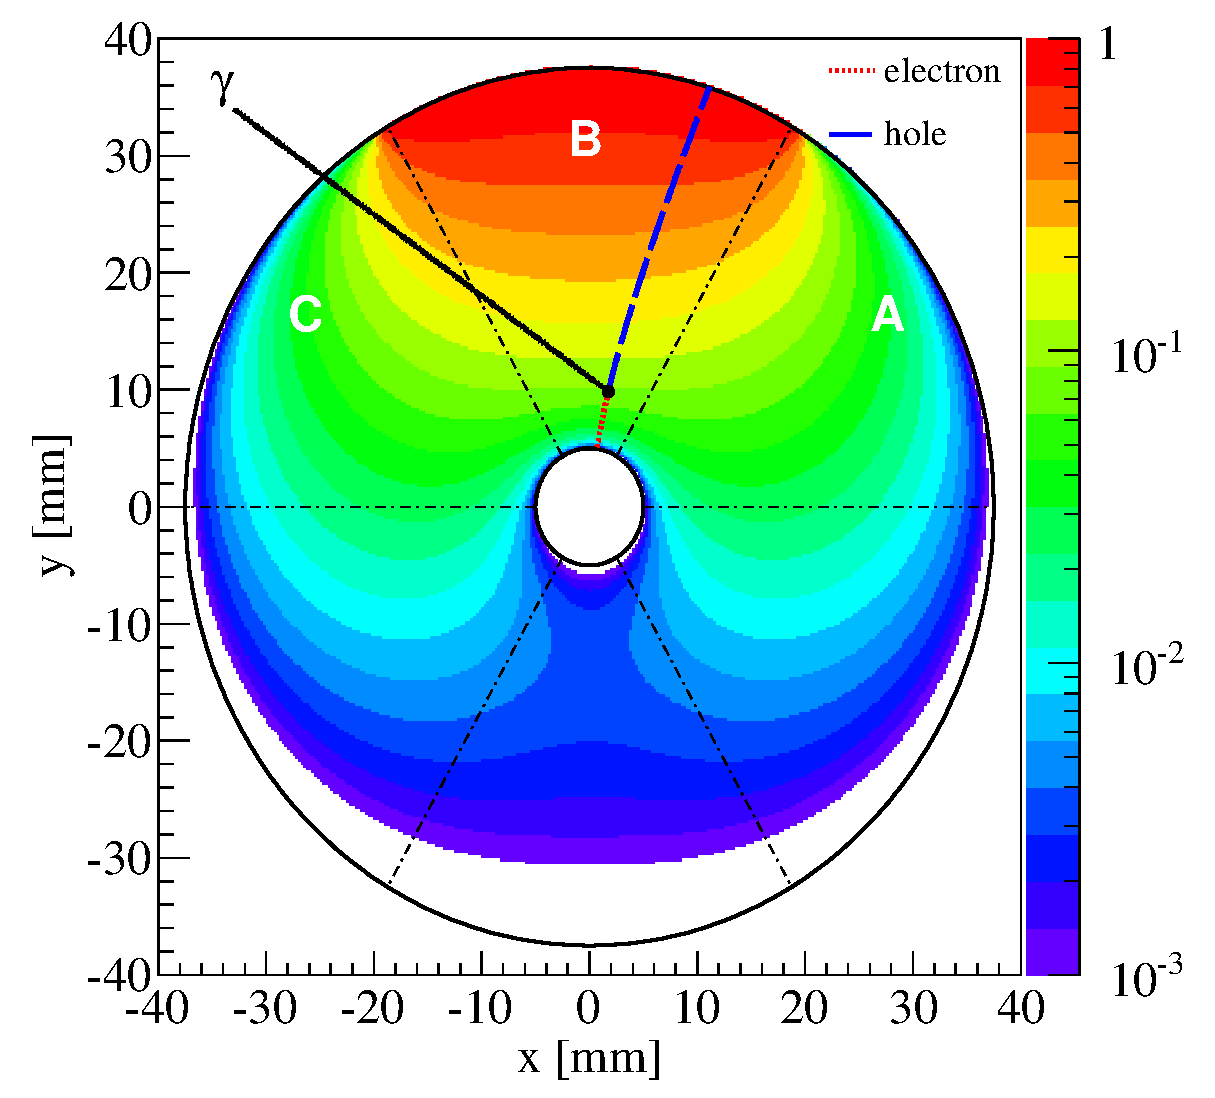
\includegraphics[height=0.22\textheight]{WP}}% 
\subfloat[]{\label{fig:det:pss} 
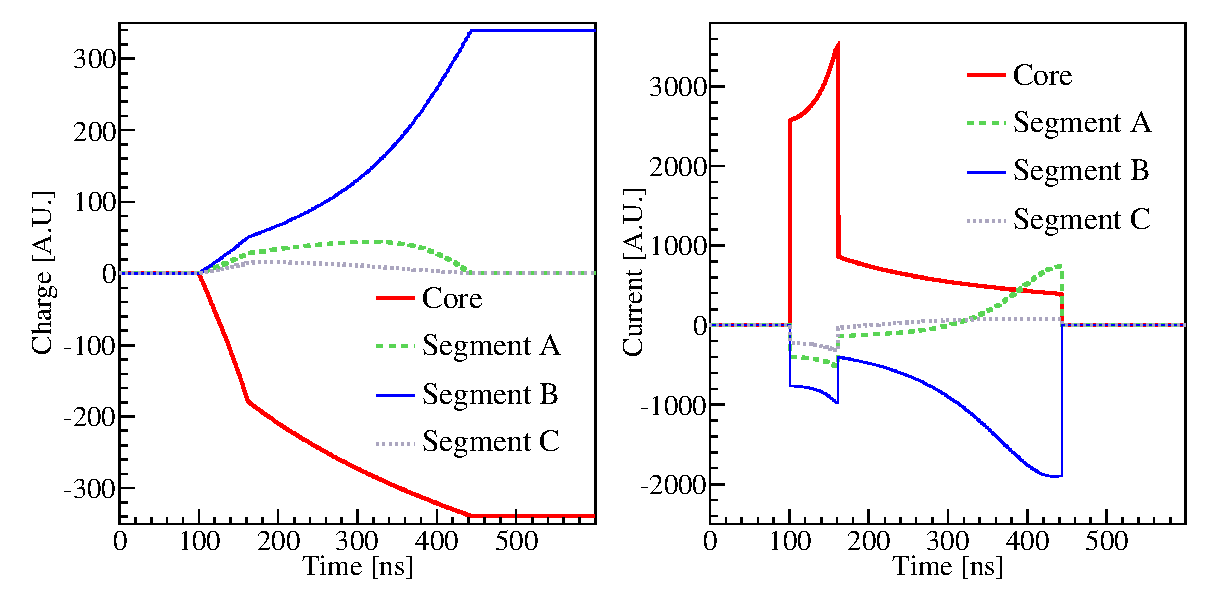
\includegraphics[height=0.22\textheight]{CIPS}}% 
\caption{(a) weighting potential of segment B together with an
indication of a $\gamma$ interaction. (b) Simulated charge and current
pulses induced in segments A, B and C.}
\label{fig:pss:ps} 
\end{figure} 

\section{Electronics}
\label{sec:det:elec}

\subsection{Noise}
\label{sec:det:noise}
The total energy resolution in terms of the full width at half maximum
(FWHM) of the peak under study, $W_{T}$, is composed of three terms:
\begin{equation}
W_{T}^{2} = W_{D}^{2} + W_{X}^{2} + W_{E}^{2},
\end{equation}
where $W_{D}$ describes the statistical fluctuations of the creation
of electron-hole pairs, $W_{X}$ describes the effect of incomplete
charge collection and scales linearly with the incident energy, and
$W_{E}$ accounts for noise contributions from the electronics and does
not depend on energy. Given a perfect electronic system, germanium
detectors have an energy resolution of about 2~keV at 1.3~MeV, where
$W_{X}$ dominates the contribution and $W_{D}$ contributes less than
1~keV. These two contributions cannot be reduced. In reality, thermal
noise in the pre-amplifiers and noise picked up by the cables and
connectors contribute significantly to the total noise. These
contributions have to be kept as small as possible.

\subsection{Cross talk}
\label{sec:det:xtalk}
For segmented germanium detectors, signals from all the electrodes are
read out simultaneously. There is intrinsic cross talk between
different channels because of the capacitive couplings between
electrodes. This cross talk is not due to improper electric
connections, hence cannot be avoided. However, it can be reduced to
an acceptable level by choosing proper values of resistors and
capacitors used in the pre-amplifier coupling and feed-back circuits
to match the intrinsic capacities between detector electrodes. A
detailed analysis is found in Chapter 4 of Ref.~\cite{Bru06} and
references therein.

%%% Local Variables:
%%% mode:latex
%%% TeX-master: "thesis"
%%% End:
